\chapter{Prečno preverjanje} 
\label{ch:precno-preverjanje}

Ocena točnosti je odvisna od podatkov v obeh podmnožicah. Da bi povečali robustnost ocene, lahko ta postopek ponovimo večkrat, vsakič z drugačno testno podmnožico. Ena takih metod je prečno preverjanje. V Orangeu je na voljo v gradniku \widget{Test and Score}.

\begin{marginfigure}
    \centering
    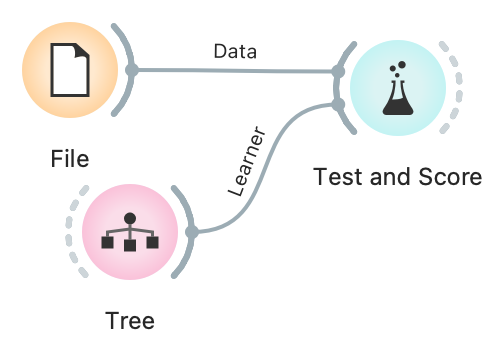
\includegraphics[width=55mm]{workflow.png}
    \caption{$\;$}
    \label{fig:workflow1}
\end{marginfigure}

V vsaki ponovitvi bo Test and Score vzel del podatkov za učenje, zgradil napovedni model na njih z izbrano metodo in potem preveril točnost modela na preostali, testni množici. Za to bo gradnik potreboval na vhodu podatke, iz katerih bo vzorčil učno in testno množico, in pa učno metodo, ki jo bo uporabil na učnih podatkih za grajenje napovednega modela. V Orangeu učnim metodam pravimo kar učenci (ang. learner). Torej Test and Score potrebuje učenca na vhodu.

\marginnote{Za tehnične tipe: učenec je objekt, ki ob prisotnosti vhodnih podatkih vrne model. Točno to, kar Test and Score potrebuje.}To je nov način, kako uporabiti gradnik \widget{Tree}. V prejšnjih delotokih smo uporabili gradnikov drug izhod, imenovan \textit{Model}; njegova gradnja je zahtevala podatke. Tokrat podatkov ne potrebuejmo; potrebujemo zgolj učenca.

Tako izgleda Test and Score gradnik. CA pomeni klasifikacijsko točnost in zaenkrat je to vse, kar nas zanima. \marginnote{Prečno preverjanje razdeli podatke na, recimo, 10 ločenih podmnožic, ki jim bomo rekli zavihki. V vsaki iteraciji se en zavihek uporabi za testiranje, ostalih 9 pa za učenje. Na ta način bo model preverjal vsak primer le enkrat.}

\begin{figure}[h]
    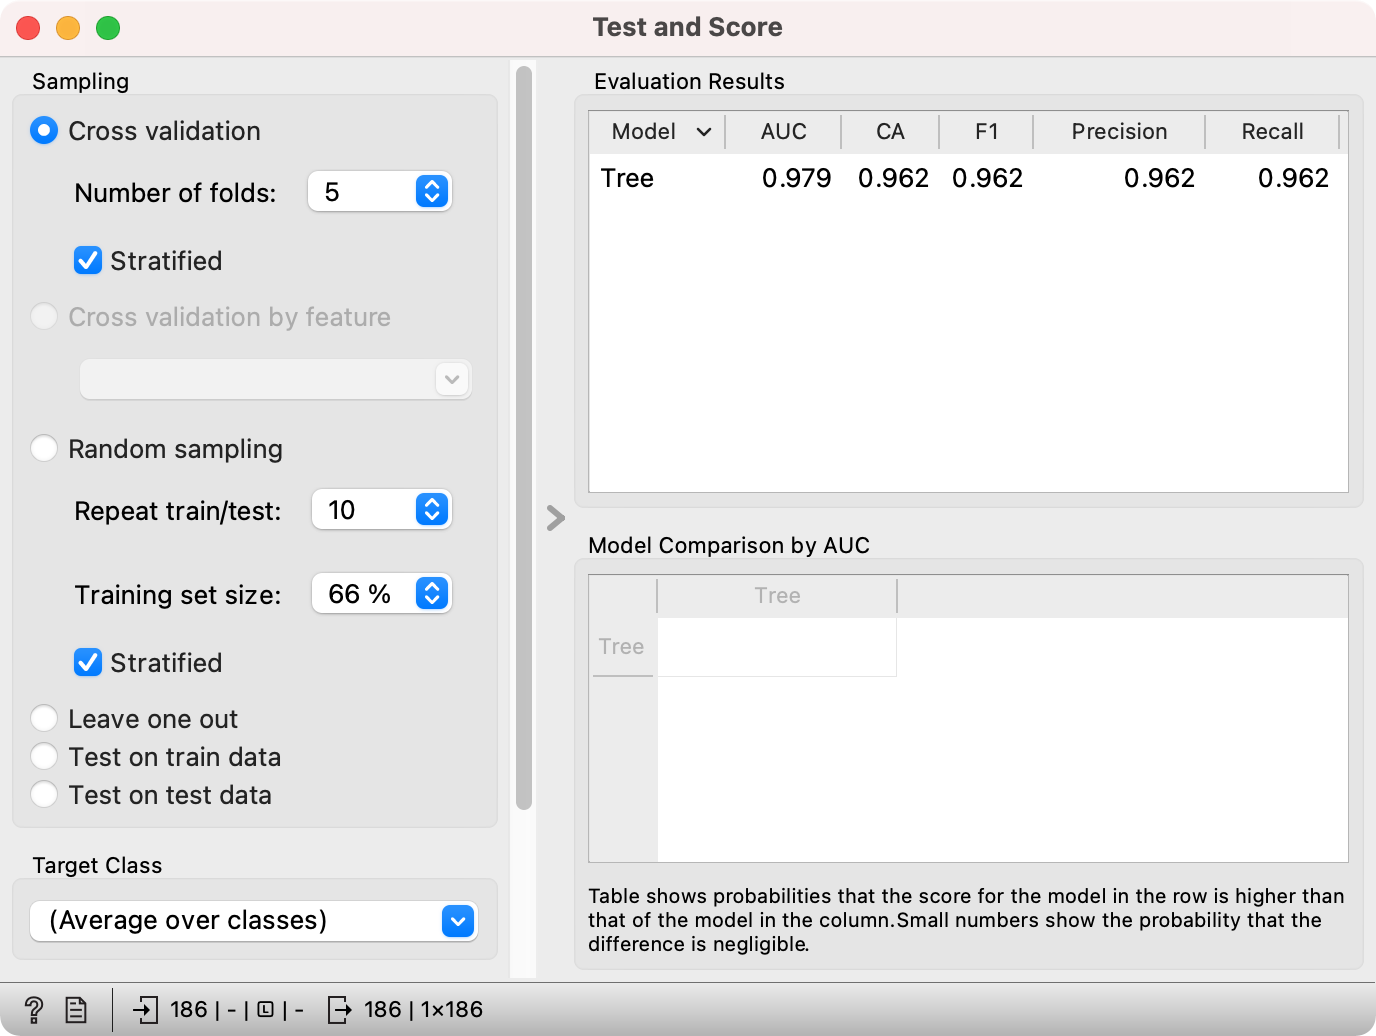
\includegraphics[width=\linewidth]{testandscore.png}
    \caption{$\;$}
\end{figure}
